\documentclass[a4paper,10pt,ngerman]{scrartcl}
\usepackage{babel}
\usepackage[T1]{fontenc}
\usepackage[utf8x]{inputenc}
\usepackage[a4paper,margin=2.5cm,footskip=0.5cm]{geometry}

\newcommand{\Aufgabe}{Aufgabe2: Verzinkt} 
\newcommand{\TeamId}{00382}
\newcommand{\TeamName}{Sehr gutes BWINF Team} 
\newcommand{\Namen}{Paul Franosch, Joshua Benning, Lenny Schürer, Marinus Lentile}          
 
\usepackage{scrlayer-scrpage, lastpage}
\setkomafont{pageheadfoot}{\large\textrm}
\lohead{\Aufgabe}
\rohead{Team-ID: \TeamId}
\cfoot*{\thepage{}/\pageref{LastPage}}

\usepackage{titling}
\setlength{\droptitle}{-1.0cm}

\usepackage{amsmath}
\usepackage{amssymb}
\usepackage{graphicx}
\usepackage{algpseudocode}

% Für Quelltext
\usepackage{listings}
\usepackage{color}
\definecolor{mygreen}{rgb}{0,0.6,0}
\definecolor{mygray}{rgb}{0.5,0.5,0.5}
\definecolor{mymauve}{rgb}{0.58,0,0.82}
\lstset{
  keywordstyle=\color{blue},commentstyle=\color{mygreen},
  stringstyle=\color{mymauve},rulecolor=\color{black},
  basicstyle=\footnotesize\ttfamily,numberstyle=\tiny\color{mygray},
  captionpos=b, % sets the caption-position to bottom
  keepspaces=true, % keeps spaces in text
  numbers=left, numbersep=5pt, showspaces=false,showstringspaces=true,
  showtabs=false, stepnumber=2, tabsize=2, title=\lstname
}
\lstdefinelanguage{JavaScript}{ % JavaScript ist als einzige Sprache noch nicht vordefiniert
  keywords={break, case, catch, continue, debugger, default, delete, do, else, finally, for, function, if, in, instanceof, new, return, switch, this, throw, try, typeof, var, void, while, with},
  morecomment=[l]{//},
  morecomment=[s]{/*}{*/},
  morestring=[b]',
  morestring=[b]",
  sensitive=true
}

% Diese beiden Pakete müssen zuletzt geladen werden
%\usepackage{hyperref} % Anklickbare Links im Dokument
\usepackage{cleveref}

% Daten für die Titelseite
\title{\textbf{\Huge\Aufgabe}}
\author{\LARGE Team-ID: \LARGE \TeamId \\\\
	    \LARGE Team-Name: \LARGE \TeamName \\\\
	    \LARGE Bearbeiter/-innen dieser Aufgabe: \\ 
	    \LARGE \Namen\\\\}
\date{\LARGE\today}

\usepackage{graphicx}
\graphicspath{ {./} }

\begin{document}

\maketitle
\tableofcontents

\section{Lösungsidee}

Ziel ist es, dass Wachstum von Kristallen nach den gegebenen Bedingungen zu simulieren. Dazu wird ein initial leeres zweidimensionales Array (Canvas) verwendet, in dem sich Keime ausbreiten. Die Wachstumsgeschwindigkeit in eine bestimmte Richtung wird dabei durch eine Wahrscheinlichkeit modelliert (Ob bei einem "Wachstumsschritt" der Keim in diese Richtung wächst). Das Wachstum erfolgt dabei rekursiv, Pixel die also durch einen wachsenden Keim eingenommen wurden, werden zu Keimen. Daten wie die Farbe und die Wachstumsgeschwindigkeiten werden dabei weitergegeben. Keime die sich nicht weiter ausbreiten können, verbleiben als gefärbte Pixel werden aber nicht weiter betrachtet.


\section{Umsetzung}
\subsection{Leinwand und Pixel}
Die Implementation erfolgt in Java.
Das Canvas wird dabei durch ein zweidimensionales Pixel Array dargestellt. Ein Pixel kann dabei EMPTY, ACTIVE oder INACTIVE sein.\\
EMPTY entspricht dem Ursprungszustand, der Pixel ist nicht gefärbt und gehört auch keinem Kristall an. ACTIVE beschreibt einen Keim / einen Pixel der noch weiter wachsen kann, INACTIVE einen gefärbten Pixel, der nicht weiter wachsen kann.\\
Außerdem besitzt jeder Pixel 4 Wachstumsgeschwindigkeiten (Richtungen auf dem Raster; Norden, Westen, Süden, Osten). Diese Wachstumsgeschwindigkeiten werden durch eine Fließkommazahl zwischen 0 und 1 dargestellt und beschreiben die Wahrscheinlichkeit, dass ein Kristall / Pixel bei einer Wachstumsiteration in diese Richtung wächst. \\
Breitet sich ein Pixel aus, gibt er all seine Daten (Farbe und Wachstumsgeschwindigkeit) weiter.
\subsection{Wachstumsprozess}
Entsteht ein neuer Kristall, erhält er eine zufällige Ausrichtung von 0 bis 1. Mit der Ausrichtung als Weißanteil wird dem Kristall dann eine Farbe der Schwarz-Weiß-Skala zugeordnet. Die Wachstumsgeschwindigkeiten werden zufällig, anhand von festgelegten Bereichen, ausgewählt. Dieser neue Pixel wird dann in eine Queue hinzugefügt und nach dem Prinzip "First in first out" abgearbeitet. Landet ein Pixel P in dieser Queue an erster Stelle, wird seine Von-Neumann-Nachbarschaft (Direkte Nachbarschaft; links, rechts, oben, unten; nicht diagonal) überprüft. Wenn ein Nachbar N den Status EMPTY hat wird N (mit der entsprechenden Wachstumsgeschwindigkeit) ACTIVE und wird an die Queue angefügt. N übernimmt dabei die Farbe und Wachstumsgeschwindigkeiten von P. \\
Sollte die gesamte Van-Neumann-Nachbarschaft keine EMPTY Pixel enthalten, wird P INACTIVE. \\
Dieser Prozess wird solange durchgeführt, bis das gesamte Canvas durch Kristalle gefüllt wurde.
\subsection{Anpassung der Ergebnisse}
Die Bildgenerierung kann dabei durch Parameter angepasst werden \\
\begin{tabular}{|p{3cm}|p{13cm}|}
\hline 
\rule[-1ex]{0pt}{2.5ex} Argument & Beschreibung \\ 
\hline 
\rule[-1ex]{0pt}{2.5ex} -width & Ganzzahl, Breite des Canvas \\ 
\hline 
\rule[-1ex]{0pt}{2.5ex} -height & Ganzzahl, Höhe des Canvas \\ 
\hline 
\rule[-1ex]{0pt}{2.5ex} -type & 'PNG' oder 'GIF', Ausgabeformat \\ 
\hline 
\rule[-1ex]{0pt}{2.5ex} -initialSP & Ganzzahl, Beschreibt die initiale Anzahl an Keimen \\ 
\hline 
\rule[-1ex]{0pt}{2.5ex} -SPperTick & Ganzzahl, Keime die pro Tick hinzugefügt werden \\ 
\hline 
\rule[-1ex]{0pt}{2.5ex} -tickDuration & Ganzzahl, Gibt an wie viele Wachstumsiterationen durchgeführt werden bevor -SPperTick Keime hinzugefügt werden \\ 
\hline 
\rule[-1ex]{0pt}{2.5ex} -minSpeedX und -maxSpeedX & Fließkommazahl, X entspricht dabei der Himmelsrichtung auf dem Canvas (N,S,W,E). Beispiel: -minSpeedN 0.1 -maxSpeedN 0.7 $\rightarrow$ Wachstumsgeschwindigkeit nach oben variiert zwischen 0.1 und 0.7 \\ 
\hline 
\rule[-1ex]{0pt}{2.5ex} -minSpeedXY und -maxSpeedXY & Fließkommazahl, X und Y entpsprechen dabei einer Himmelsrichtung auf dem Canvas (N,S,W,E). So kann die Geschwindigkeit einer "Achse" einfacher angegeben werden Beispiel: -minSpeedNS 0.1 -maxSpeedNS 0.7 \\ 
\hline 
\end{tabular} \\
\subsection{Ausgabe}
Die Ausgabe der Muster erfolgt entweder als PNG oder GIF. Das Programm legt dazu einen Ordner "out" an und speichert dort entsprechende Dateien ab. Im Folgenden wird auf die Einstellung der Parameter anhand der Bilder eingegangen, im Anhang finden sich aber auch GIFs mit ähnlichen Parametern wie die Beispiele.


\section{Beispiele}
\subsection{Initiale Keime und Wachstumsgeschwindigkeiten}
\centerline{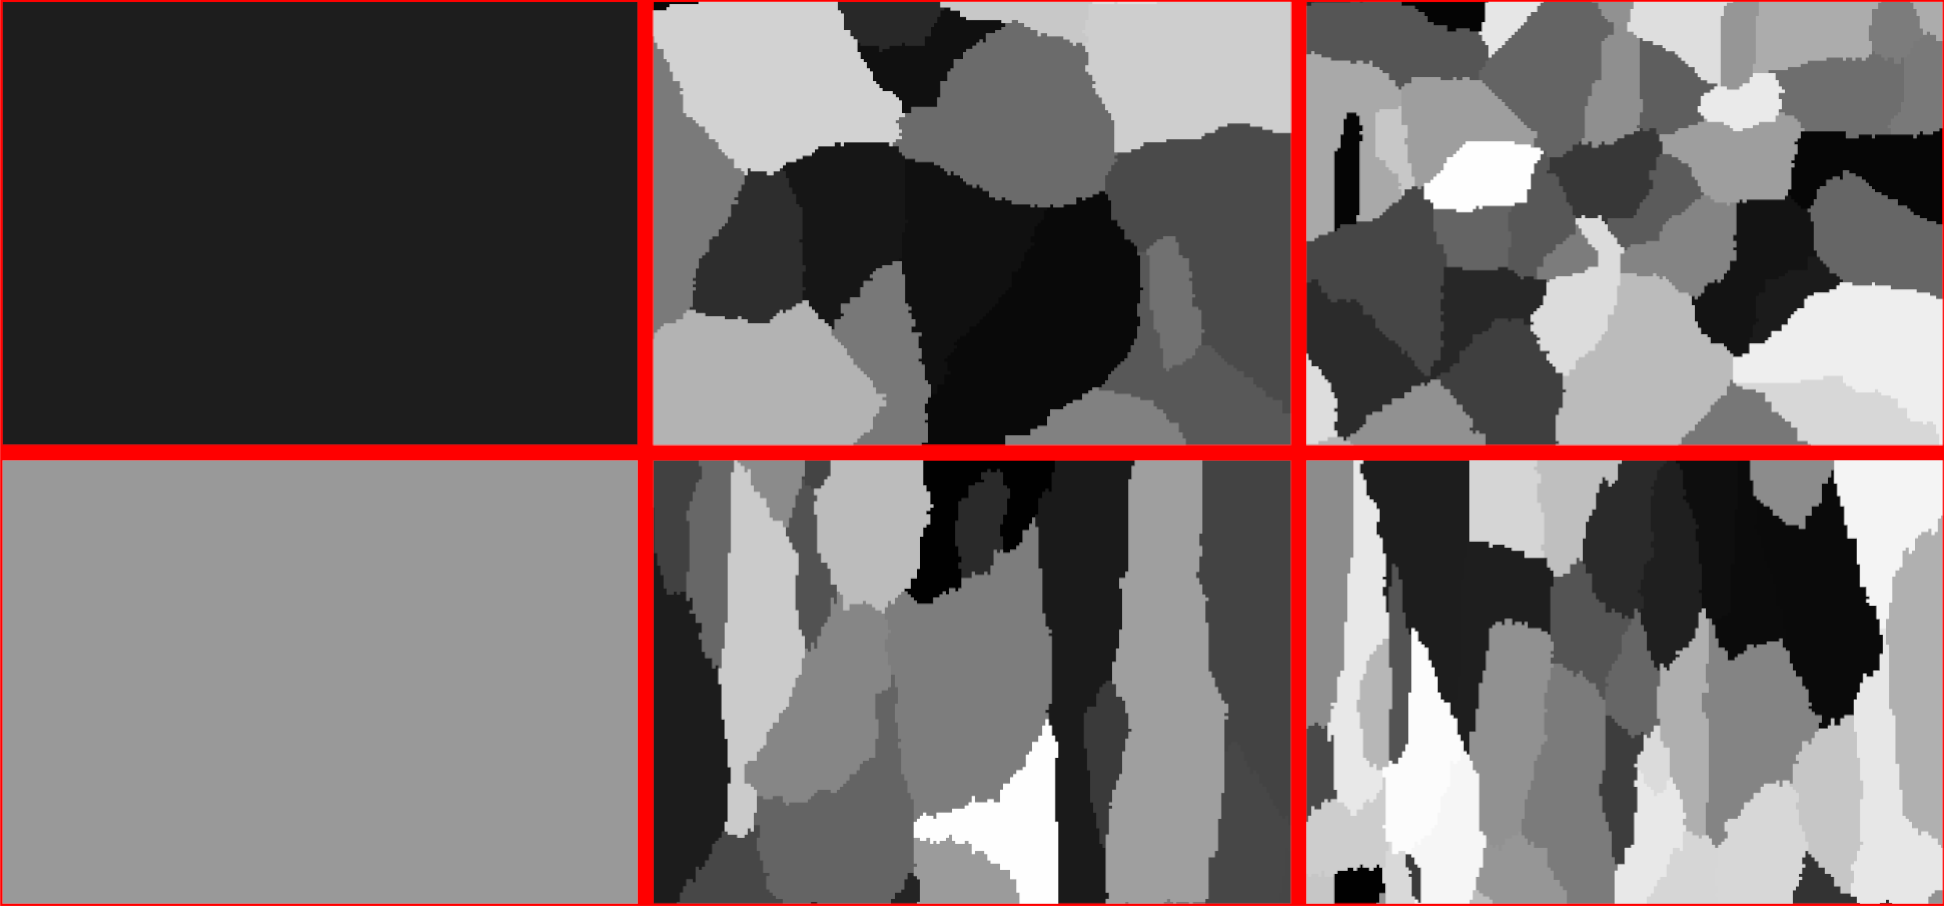
\includegraphics{collage2}}
Bei einem Canvas von 200px x 200px sind hier Muster mit links einem, in der Mitte 25 und rechts 50 initialen Keimen dargestellt. Hier wird allerdings deutlich, dass da die einzelnen Kristalle ähnlich groß sind das Referenzbild nur schwer anzunähern ist.
Bei der oberen Reihe variieren dabei die Wachstumsgeschwindigkeiten in alle Richtungen von 0.0 bis 1.0. Bei der unteren wurden für die Ost-West-Achse ein Maximum von 0.1 festgelegt. Die Kristalle werden daher bis zu 10x höher als sie breit sind.
\subsection{Späteres Hinzufügen von Keimen}
\centerline{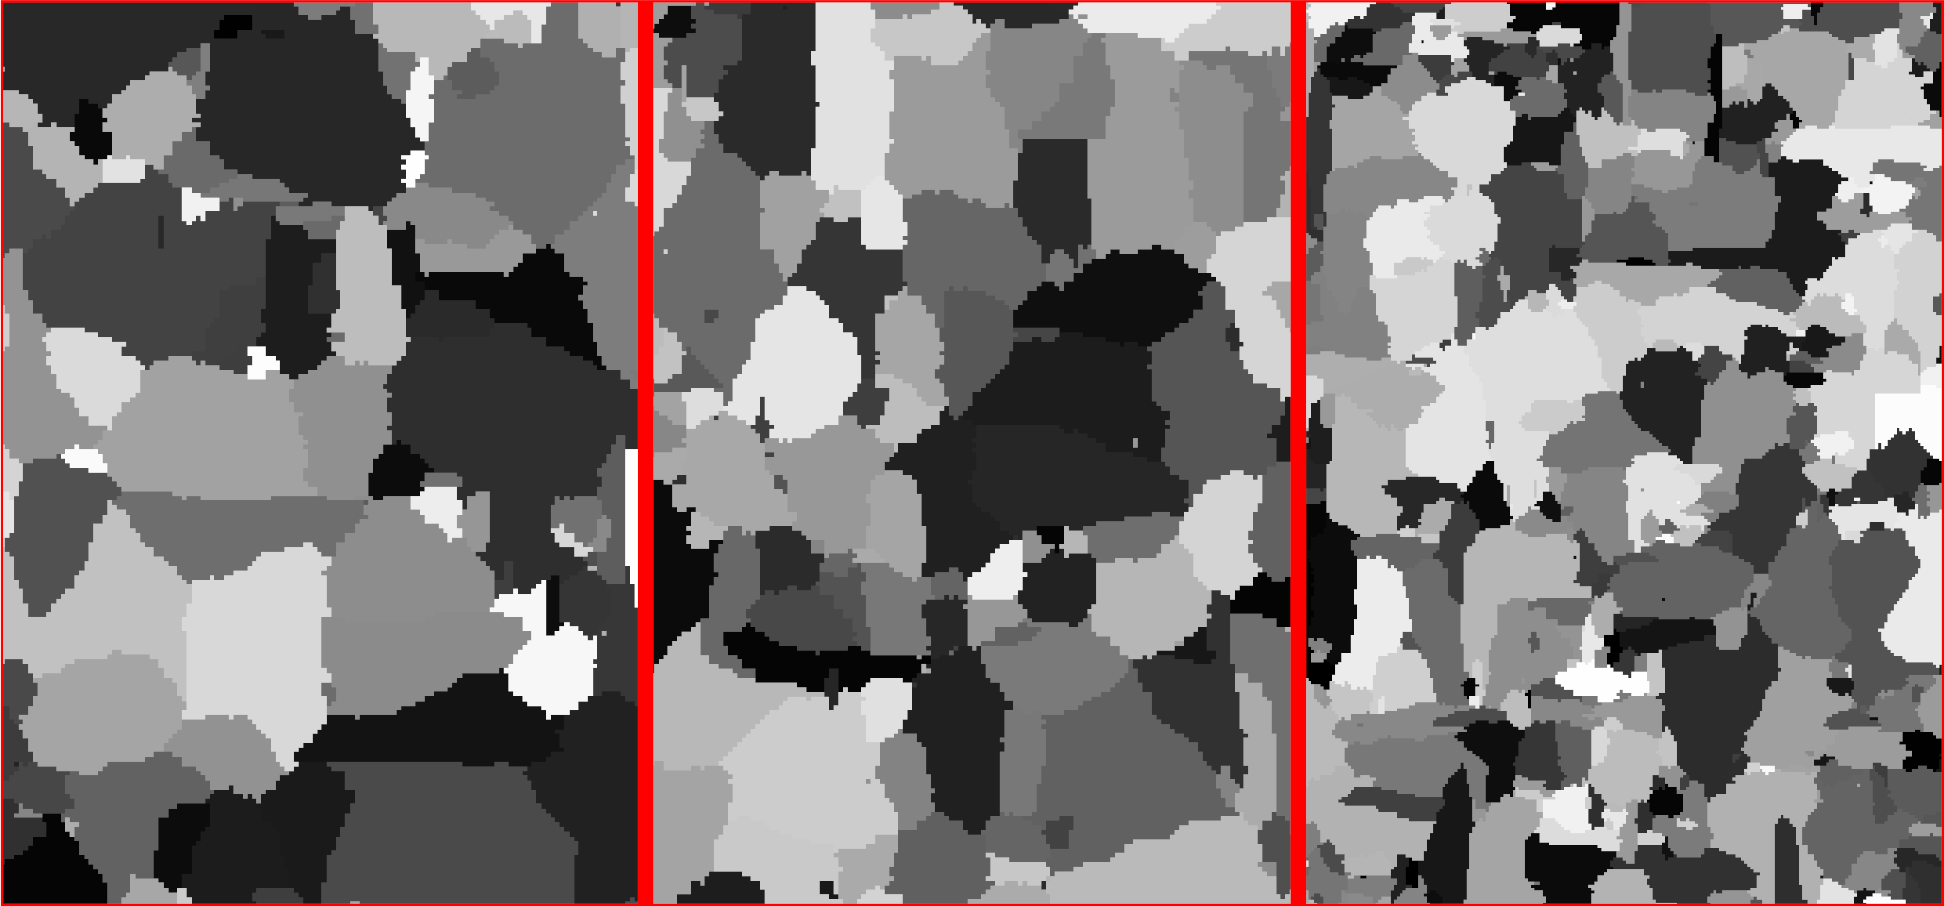
\includegraphics{collage1}}
Da auf dem Referenzbild allerdings Kristalle verschiedener Formen und allgemein verschiedener Größen vorliegen, reichen die Wachstumsgeschwindigkeit und die Keimzahl nicht, um diese Varianz vollständig darzustellen. Es bietet sich daher an, Keime erst auf das Raster zu setzen nachdem andere bereits Zeit zum Wachsen hatten.
In den Beispielen hier wurde wieder ein Raster von 200px x 200px verwendet. In dem Bild links wurde 1 Keim, im Mittleren wurden 15 Keime und rechts wurden 30 Keime pro 3 Wachstumsiterationen hinzugefügt. Die Bilder hier ähneln dem Referenzbild schon eher, da sie sowohl Bereiche mit Ansammlungen kleiner als auch große, durchgängige Kristalle aufweisen.
\subsection{Beispiele}
\subsubsection{Beispiel 1}
\centerline{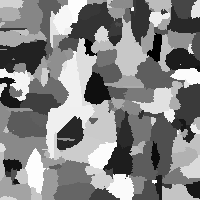
\includegraphics{beispiel1}}
\subsubsection{Beispiel 2}
\centerline{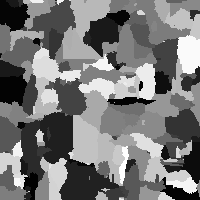
\includegraphics{beispiel2}}
\subsubsection{Beispiel 3}
\centerline{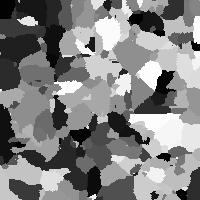
\includegraphics{beispiel3}}
\newpage
\subsubsection{Beispiel 4}
\centerline{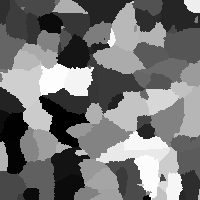
\includegraphics{beispiel4}}
\subsubsection{Beispiel 5}
\centerline{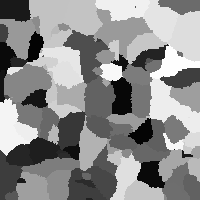
\includegraphics{beispiel5}}

\newpage
\section{Quellcode}
\subsection{ImageGenerator-Klasse}
\begin{lstlisting}[language=Java]
public class ImageGenerator {
    private final ImageGenData imageGenData;
    private final GrowSpeedGenerator growSpeedGenerator;
    private final GenerationData generationData; // Done

    private List<BufferedImage> images = new ArrayList<>();

    public void generateImage() throws IOException {
        Long start = System.currentTimeMillis();
        try {
            String d = getProgramPath() + "/out/";
            File dir = new File(d);
            if (dir.exists()) System.out.println("Output folder was found");
            if (!dir.mkdir()) System.out.println("Could not generate output folder!");
        }
        catch (Exception e) { System.out.println("Exception occured" + e);}


        Canvas canvas = new Canvas(imageGenData.getWidth(), imageGenData.getHeight(), Color.BLACK);
        Random random = new Random();
        Queue<Pixel> pixelsToExpand = new ConcurrentLinkedQueue<>(); // Pixels that can grow
        generateStartPoints(canvas, random, pixelsToExpand,  generationData.getInitialSP());
        int iterationCount = 0; // Counting iterations
        while (pixelsToExpand.size() != 0 && iterationCount < 1_000_000) {
            if (iterationCount % generationData.getTickDuration() == 0) 
            	generateStartPoints(canvas, random, pixelsToExpand, generationData.getSPperTick());
            
            Pixel poll = pixelsToExpand.poll();
            if (poll != null) poll.setPixelState(Pixel.PixelState.INACTIVE);
            pixelsToExpand.addAll(canvas.expand(poll));
            iterationCount++;

            // Saving a frame every 1000 iterations if a GIF should be generated
            if (this.imageGenData.getImageType() == ImageType.GIF && iterationCount % 1000 == 0) {
                images.add(canvas.render(false, ""));
            }
        }
    }

    
    private void generateStartPoints(Canvas canvas, Random random, 
    															Queue<Pixel> pixelsToExpand, int count) {
        for (int spawnPoint = 0; spawnPoint < count; spawnPoint++) {
            int w = random.nextInt(this.imageGenData.getWidth());
            int h = random.nextInt(this.imageGenData.getHeight());
            Pixel startPxl = canvas.getData()[w][h];
            if (startPxl.getPixelState() != Pixel.PixelState.EMPTY) {
                spawnPoint--;
                continue;
            }
            int rgbValue = (int) (random.nextFloat(0.0f, 1.0f) * 255);
            startPxl.setColor(new Color(rgbValue, rgbValue, rgbValue));
            startPxl.setGrowSpeed(this.growSpeedGenerator.getRandomSpeed());
            startPxl.setPixelState(Pixel.PixelState.INACTIVE);
            pixelsToExpand.add(startPxl);
        }
    }
}
\end{lstlisting}

\newpage
\subsection{Canvas-Klasse}
\begin{lstlisting}[language=Java]
public class Canvas {
    private final Pixel[][] data;
    private final int width;
    private final int height;

    public Canvas(int width, int height, Color defaultColor) {
        this.data = new Pixel[width][height];
        this.width = width;
        this.height = height;
        for (int x = 0; x < this.width; x++) {
            for (int y = 0; y < this.height; y++) {
                this.data[x][y] = new Pixel(x, y, Pixel.PixelState.EMPTY, defaultColor);
            }
        }
    }

    public Pixel[][] getData() {
        return data;
    }

    public HashMap<Pixel.Direction, Pixel> getNeumannNeighbours(Pixel pixel) {

        HashMap<Pixel.Direction, Pixel> neumannNeighbours = new HashMap<>();

        int x = pixel.getX();
        int y = pixel.getY();

        if (x + 1 < this.width) neumannNeighbours.put(Pixel.Direction.EAST, this.data[x + 1][y]);
        else neumannNeighbours.put(Pixel.Direction.EAST, null);
        if (x - 1 >= 0) neumannNeighbours.put(Pixel.Direction.WEST, this.data[x - 1][y]);
        else neumannNeighbours.put(Pixel.Direction.WEST, null);
        if (y + 1 < this.height) neumannNeighbours.put(Pixel.Direction.NORTH, this.data[x][y + 1]);
        else neumannNeighbours.put(Pixel.Direction.NORTH, null);
        if (y - 1 >= 0) neumannNeighbours.put(Pixel.Direction.SOUTH, this.data[x][y - 1]);
        else neumannNeighbours.put(Pixel.Direction.SOUTH, null);

        return neumannNeighbours;
    }

    public HashMap<Pixel.Direction, Pixel> getEmptyNeighbours(Pixel pixel) {
        HashMap<Pixel.Direction, Pixel> neumannNeighbours = getNeumannNeighbours(pixel);
        HashMap<Pixel.Direction, Pixel> emptyNeumannNeighbours = new HashMap<>(neumannNeighbours);
        for (Map.Entry<Pixel.Direction, Pixel> directionPixelEntry : neumannNeighbours.entrySet()) {
            Pixel value = directionPixelEntry.getValue();
            if (value != null && value.getPixelState() != Pixel.PixelState.EMPTY) {
                emptyNeumannNeighbours.remove(directionPixelEntry.getKey());
            }
        }
        return emptyNeumannNeighbours;
    }

    public List<Pixel> expand(Pixel pixel) {
        List<Pixel> newPixel = new ArrayList<>();
        Random random = new Random();
        for (Pixel.Direction value : Pixel.Direction.values()) {
            Pixel neumannNeighbour = this.getEmptyNeighbours(pixel).get(value);
            if (neumannNeighbour != null) {
                if (random.nextFloat() < pixel.getGrowSpeed().get(value)) {
                    neumannNeighbour.setColor(pixel.getColor());
                    neumannNeighbour.setPixelState(Pixel.PixelState.ACTIVE);
                    neumannNeighbour.setGrowSpeed(pixel.getGrowSpeed());
                    newPixel.add(neumannNeighbour);
                } else { // Pixel would be fillable, but was not due to the growSpeed
                    newPixel.add(pixel); // Pixel will be expanded another time
                }
            }
        }
        return newPixel;
    }

    public BufferedImage render(boolean saveFile, String fileName) {
        BufferedImage image = new BufferedImage(this.width, this.height, BufferedImage.TYPE_INT_RGB);
        int total = 0;
        for (int x = 0; x < this.width; x++) {
            for (int y = 0; y < this.height; y++) {
                if (this.data[x][y].getPixelState() == Pixel.PixelState.ACTIVE) {
                    image.setRGB(x, y, this.data[x][y].getColor().getRGB());
                    total++;
                } else if (this.data[x][y].getPixelState() == Pixel.PixelState.INACTIVE) {
                    Color pixelColor = this.data[x][y].getColor();
                    image.setRGB(x, y, 
                    	new Color(pixelColor.getRed(), 
                    				pixelColor.getGreen(), 
                    				pixelColor.getBlue()).getRGB());
                    total++;
                }
            }
        }
        try {
             if (saveFile) ImageIO.write(image, "PNG", new File("./out/" + fileName + ".png"));
            return image;
        } catch (IOException e) {
            e.printStackTrace();
            return null;
        }
    }
}
\end{lstlisting}



\end{document}
